% tex file for hypothesis testing results

\begin{figure}[ht]

\centering

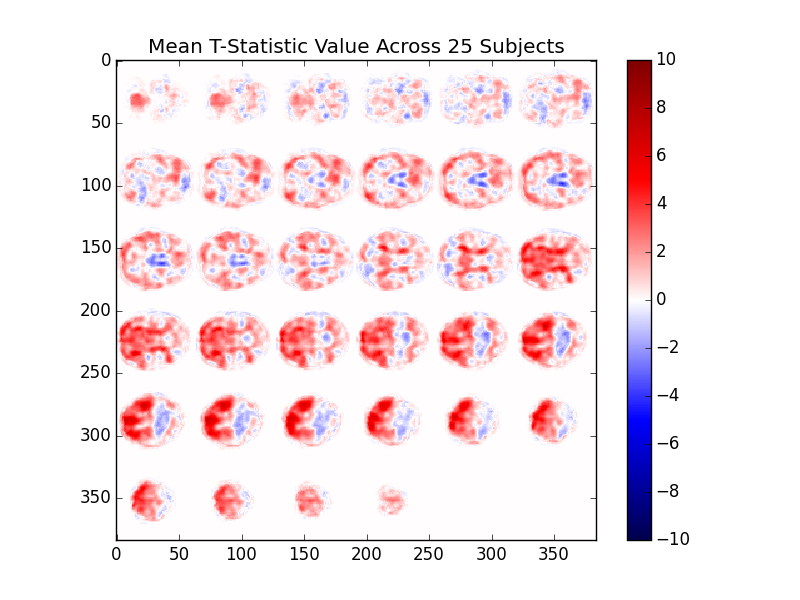
\includegraphics[scale=0.5]{images/hypothesis_testing}  

\caption{Ben sucks.}

\label{fig:mask}

\end{figure}


\par \indent We created our simple linear regression model not necessarily for prediction but rather to understand the relationship between the voxels in a subject's brain and the convolved time course. In order to measure the strength of the relationship between these two measurements, we ran a hypothesis test on the coefficient of the linear regression model.
	\par In our case, we ran a t-test on the $\beta_1$ coefficient of the model with the null hypothesis that $\beta_1=0$ and the alternative hypothesis that $\beta \neq 0$. Since there is a linear model associated with each voxel in a subject’s image, we have a single t-statistic associated to each voxel in our simple linear regression case. Once we had obtained the t-statistic, we compared this value across voxels in two ways. First, we simply compared this value across voxels in a subject. In this case, we took into account the sign of the t-statistic in our analysis. Second, we converted this t-statistic to a p-value, in which case the sign of the t-value will become irrelevant and we compared across voxels without taking into account this sign.  We also developed functions to create t-statistics for multiple feature linear regression. 
	
	\par \indent Now that we created a method to compare the voxels within a single subject, we next examined our results for the same voxels across subjects. Our initial step was to aggregate the t-statistic data between all subjects for each voxel. This allowed us to decrease the variability of the fit on each voxel and detect a more clear signal. 

	\par \indent In order to do this, we ran the hypothesis test as stated above on all 24 subjects of the study. Then per voxel, we took the simple average of these values. An issue with our data was the presence of empty space that the scanner detected that is not directly part of the brain. In order to account for this, we took the mask data of the brain and ‘cut out’ the parts of the images that were not relevant. 

[Figure \ref{fig:mask}]
